% !TEX TS-program = pdflatex
% !TEX encoding = UTF-8 Unicode

% This file is a template using the "beamer" package to create slides for a talk or presentation
% - Giving a talk on some subject.
% - The talk is between 15min and 45min long.
% - Style is ornate.

% MODIFIED by Jonathan Kew, 2008-07-06
% The header comments and encoding in this file were modified for inclusion with TeXworks.
% The content is otherwise unchanged from the original distributed with the beamer package.

\documentclass{beamer}


% Copyright 2004 by Till Tantau <tantau@users.sourceforge.net>.
%
% In principle, this file can be redistributed and/or modified under
% the terms of the GNU Public License, version 2.
%
% However, this file is supposed to be a template to be modified
% for your own needs. For this reason, if you use this file as a
% template and not specifically distribute it as part of a another
% package/program, I grant the extra permission to freely copy and
% modify this file as you see fit and even to delete this copyright
% notice. 


\mode<presentation>
{
  \usetheme{Berkeley}
  % or ...

  \setbeamercovered{transparent}
  % or whatever (possibly just delete it)
}


\usepackage[english]{babel}
% or whatever

\usepackage[utf8]{inputenc}
% or whatever

\usepackage{times}
\usepackage[T1]{fontenc}
% Or whatever. Note that the encoding and the font should match. If T1
% does not look nice, try deleting the line with the fontenc.


\title[UE PROG6] % (optional, use only with long paper titles)
{Soutenance de projet}

\subtitle
{Interface conviviale pour le jeu du Tablut} % (optional)

\author[] % (optional, use only with lots of authors)
{B.~Berkati \and E.~Berthier \and A.~Canonne \and M.~Dufrenoy \and M.~Duplan \and L.~Postic}
% - Use the \inst{?} command only if the authors have different
%   affiliation.

\institute[Universities of Somewhere and Elsewhere] % (optional, but mostly needed)
{
  IM2AG - Département STS Informatique\\
  Université Joseph Fourier
 }
% - Use the \inst command only if there are several affiliations.
% - Keep it simple, no one is interested in your street address.

\date[UET Animation scientifique] % (optional)
{6 juin 2014 - IM2AG}

\subject{Talks}
% This is only inserted into the PDF information catalog. Can be left
% out. 



% If you have a file called "university-logo-filename.xxx", where xxx
% is a graphic format that can be processed by latex or pdflatex,
% resp., then you can add a logo as follows:

% \pgfdeclareimage[height=0.5cm]{university-logo}{university-logo-filename}
% \logo{\pgfuseimage{university-logo}}



% If you wish to uncover everything in a step-wise fashion, uncomment
% the following command: 

%\beamerdefaultoverlayspecification{<+->}


\begin{document}

\begin{frame}
  \titlepage
\end{frame}




% Since this a solution template for a generic talk, very little can
% be said about how it should be structured. However, the talk length
% of between 15min and 45min and the theme suggest that you stick to
% the following rules:  

% - Exactly two or three sections (other than the summary).
% - At *most* three subsections per section.
% - Talk about 30s to 2min per frame. So there should be between about
%   15 and 30 frames, all told.

\section{Introduction}

\begin{frame}{Introduction}
  \tableofcontents
  % You might wish to add the option [pausesections]
\end{frame}

\section{Contexte du projet}

\subsection{Le Tablut}

\begin{frame}{Le Tablut}{La famille des jeux de Tafl}
  \begin{itemize}
  \item Un plateau de jeu carré
	\item Des cases marquées symétriquement
	\item Des forces inégales
	\item Un principe de prise par encadrement
	\item Des objectifs de jeux différents
	\item Une pièce particulière, le Roi
  \end{itemize}
\end{frame}

\begin{frame}{Le Tablut}{Le plateau de jeu}
 \begin{center}
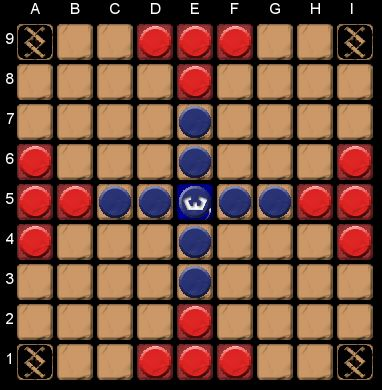
\includegraphics[width=6cm]{plateau.jpg}
\end{center}
\end{frame}

\subsection{Choix de la technologie}

\begin{frame}{Choix de la technologie}{LibGDX}
  \begin{itemize}
  \item Plusieurs plates-formes, un seul code
	\item Performant
	\item Très documenté
	\item Nombreux widgets disponible
	\item Open Source
  \end{itemize}
\end{frame}

\section{Réalisation technique globale}

\begin{frame}{Réalisation technique globale}{Modèle-Vue-Controlleur}
 \begin{center}
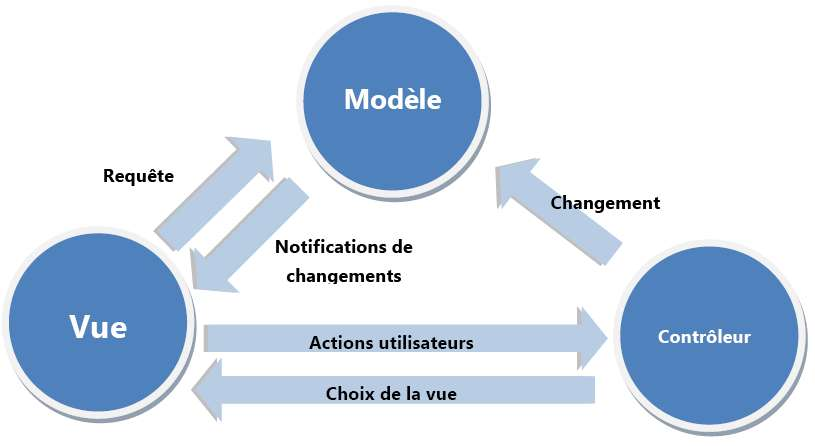
\includegraphics[width=10cm]{mvc.jpg}
\end{center}

\end{frame}

\begin{frame}{Réalisation technique globale}{Architecture globale}
\begin{center}
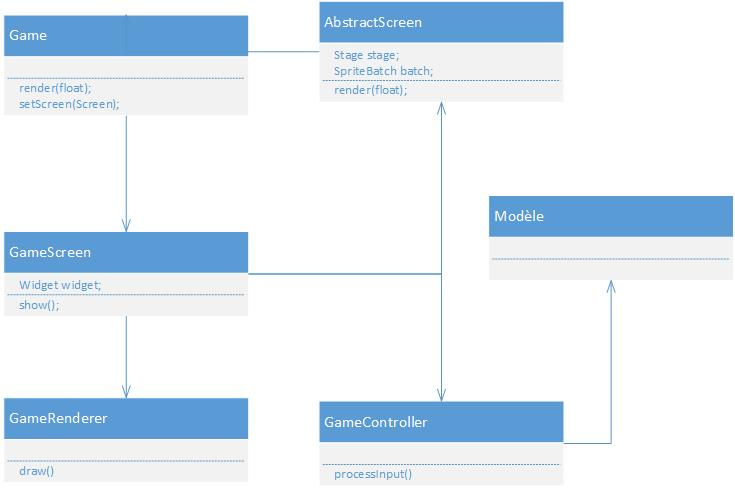
\includegraphics[width=10cm]{uml.jpg}
\end{center}

\end{frame}

\begin{frame}{Réalisation technique globale}{Widgets personnalisés}
 \begin{itemize}
  \item Indicateur de l'état du jeu
	\item Historique des coups
	\item Sélecteur des paramètres du joueur
	\item Sélecteur des paramètres de la partie
 \end{itemize}
\end{frame}

\section{IHM}

\begin{frame}{IHM}{Conception}
 \begin{itemize}
  \item Inspiration de jeu existant
	\item Historique des coups
	\item Sélecteur des paramètres du joueur
	\item Sélecteur des paramètres de la partie
 \end{itemize}
\end{frame}

\begin{frame}{IHM}{Validation}
 \begin{itemize}
  \item En interne : de manière empirique
	\item En réunion : retour des professeurs
	\item En externe : week-end de bêta-test
 \end{itemize}
\end{frame}

\begin{frame}{IHM}{Echantillon de la bêta-test}
 \begin{center}
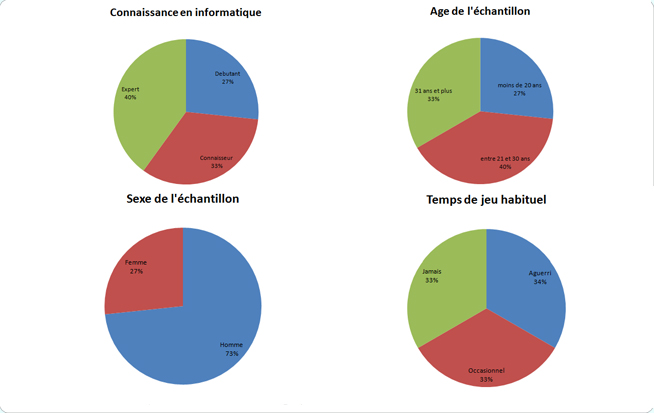
\includegraphics[width=6cm]{echantillon.jpg}
\end{center}
\end{frame}

\begin{frame}{IHM}{Résultat de la bêta-test}
 \begin{center}
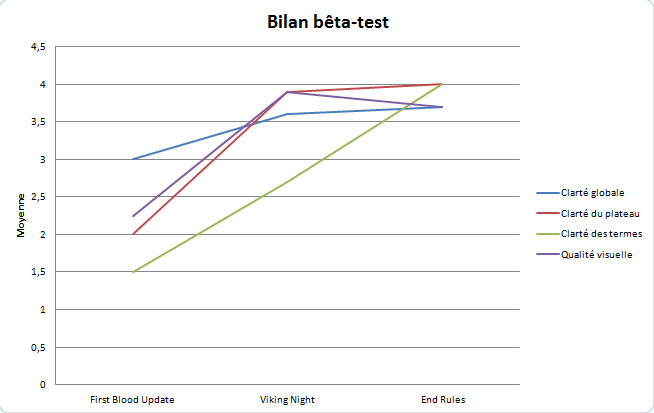
\includegraphics[width=6cm]{resBeta.jpg}
\end{center}
\end{frame}

\section{IA}


\section{Bilan}

\begin{frame}{Bilan}

  % Keep the summary *very short*.
  \begin{itemize}
  \item Les règles du jeu ont été parfaitement intégré 
  \item 
  \item 
  \end{itemize}
  
	Retrouvez le projet sur https://github.com/Foelthanos/Obichouvine.
 
\end{frame}


\end{document}


